\documentclass[a4paper,11pt]{article}

\usepackage[utf8]{inputenc}
\usepackage[english]{babel}
\usepackage{amsmath,amssymb}
\usepackage{cancel}
\usepackage{booktabs}

\usepackage{color,graphicx}

\usepackage{listings}

\author{Anders A. Søndergaard}
\title{Numerical methods project}

\begin{document}
\maketitle

\begin{abstract}
\noindent In this report a method is described for compressing sound files
using the Fast Fourier Transform. An algorithm is implemented in C,
and a few example sound files are compressed to a little less than half their
size. Some theory for further improvements and techniques
will be discussed.
\end{abstract}

\section{Theory}

A typical raw sound file consists of a series of samples,
that, when fed through a digital-analog converter at a given rate,
will give a sound signal that can be applied to a loudspeaker.

These samples can be thought of as a list of (t,x) pairs where $t$ is time and
$x$ is position.
If we take the Fourier transform of this list, we get
a list of amplitudes and frequencies (the Fourier coefficients, $c_k$).

This can be exploited to compress the sound file. The human ear
can hear frequencies in the range of roughly 60-17,000 Hz,
so if we cut away all frequency samples not in this range,
we save space. Furthermore, if the amplitude of a given frequency
is very low compared to the other samples, we can ignore it too.

This is an example of results from a field called psychoacoustics.
Other results are that the human ear masks certain frequencies when others are present,
and perceive nonexistent frequencycomponents under certain circumstances.
For example the ear will not be able to distinguish
a harmonic series where the fundamental node is missing from
one where it is present.

In this small project, we only throw away frequencies out of the 60-17000 Hz
range and frequencies of low intensity, but in the MP3 compression scheme,
as many results as possible from psychoacoustics are used.

Normally, one splits the file into time windows of some length.
There are a number of advantages of doing this in MP3 for example.
It is easier to stream the file, and you won't need to have all the raw
samples in memory. But more importantly, in MP3, the
sample waveform can be more difficult to encode
some places than others. The individual frames will then not be
affected by local difficulties.

You also get a slight speedup, as you then go from a time complexity
of  $n\log(n)$ to $n\log(w)$, where $w$ is the number of samples in each frame
and $n$ is the number of samples in the entire file.


When you split the file in frames and throw away Fourier coefficients,
some edge effects are bound to occur, because we actually take a Fourier transform
of a function folded with a square window. To counter this,
MP3 overlaps frames and use other windowing functions to smoothe
out the frame transitions. In this time constrained project,
we don't bother, and accept some clicking in the decompressed files.


To determine the frame size we're going to use (number of samples per frame),
we consider the frequency resolution needed. We (arbitrarily) set
the required resolution to 10 Hz (to be able to distinguish 60 from 70 Hz).
At least we need to be able to cut at 17000 Hz, and not 16000 Hz.
The frame size might be optimized to allow for a greater number
of samples to be thrown away, but I have not investigated this matter further.
MP3 uses a frame size of a few hundred frequency samples, but spread out
data for each position sample over multiple frames (not just the nearest neighbours).


When we choose 10 Hz resolution, we find that, since the number of samples $N = \text{Sample
Rate} \times \text{time}$, and the $k$'th fourier coefficient
corresponds to the frequency $f_k = k/2N$,
that we need a window size of at least 4410 samples if the wave file
is encoded with 44100 samples per second, as is the case in most audio CD's.
For the fast Fourier transform to be efficient,
we need some power $p$ that makes $2^p =N$. We therefore choose $p = 13$,
giving us a window size of $8192$ samples. It should be noted that
other Fast Fourier Transform algorithms have been deviced, that does
not have this requirement. Our Cooley-Tukey algorithm, for example,
can also be used to split the data into 3 or 4 or 5 and so on lower transforms, not just 2.

We throw away all (now complex) samples above $k = 1700$,
and end up with only needing to store about 58\% fewer numbers,
reducing our file to 42\% of its original size.

To improve on this number, we also throw away fourier coefficients that
have a too low amplitude. A clever algorithm could be found that determines
what too low means, but in our project we say that a minimal amplitude
of 0.01 is required to be needed. This value is experimentally found to be
the highest value that still gives a reasonable sound quality
on the authors cheap laptop loudspeakers.

When we throw away samples like this, we need a bitmap of which
samples are kept and thrown away. For the 1700 samples,
this would take up 212 bytes, equivalent to 53 complex
samples encoded with 16 bits of accuracy. We then need to throw away
at least 3\% of the remaining samples for this method to be worthwhile,
which does not seem unreasonable.


On a side note, this method alone applied to an uncompressed noisy
signal, could blank out the noise. If you know the frequency of
the noise, you can also simply remove the offending frequency from
the spectrum.


\section{WAV files}

\begin{figure}
\begin{center}
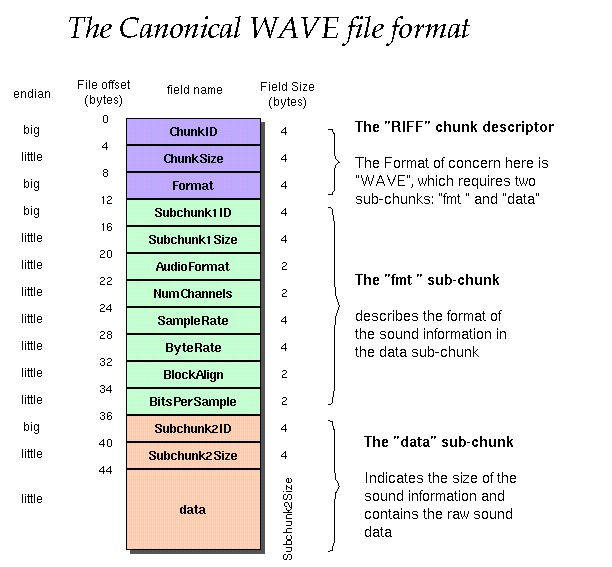
\includegraphics[width=0.75\textwidth]{wav-sound-format.jpg}
\end{center}
\caption{Canonical WAVE file format \cite{wav}}
\label{fig:wave}
\end{figure}

A WAV file is a RIFF file (binary file of chunks)
that consists of a header describing the data and the data itself
placed in the ``fmt '' and ``data'' subchunks, respectively.
The samples are stored from start to end with each channel (mono, stereo,
\ldots)
interleaved so the file can be read sequentially and still produce
samples for each channel. If there are 8 bits per sample, an offset of
127 is added, otherwise the samples are stored as regular 2's complement
signed integers.

To read these files, a simple library was written. It provides functions
for reading already existing WAV files, and functions for creating and writing
to WAV files created by the program (ie. only canonical WAV files, not
wav files with other headers).

\section{Algorithms}

For compressing WAV files, the compressor enters this
main loop
\begin{lstlisting}
while ((ReadSamples = readwav(...)) != 0) {

...

rmax = imax = 0; // Frame abs maximum real, imag part
for (n = 0; n < NumChannels; n++) {
   if (ReadSamples < NumSamples) { // Fill the rest with 0's
   for (k = ReadSamples; k < NumSamples; k++)
      channels[n][k] = 0;
   }
   // Prepare for FFT
   for (k = 0; k < NumSamples; k++) {
      channelspreFFT[n][k] = (complex) channels[n][k];
   }

   // FFT:
   fft(NumSamples, channelspreFFT[n], channelspostFFT[n], -1);

   // Readout:
   for (k = minSample; k < maxSample; k++) {
   // Check if we can throw away sample
   if (cabs(channelspostFFT[n][k]) > MIN_AMPLITUDE) {
      bitmap_handler_set(&header,k-minSample, n);

      channels[n][2*(k-minSample)] = creal(channelspostFFT[n][k]);
      channels[n][2*(k-minSample) + 1] = cimag(channelspostFFT[n][k]);

      // Check is a new maximum has been found
      if (rmax < fabs(channels[n][2*(k-minSample)]))
         rmax = fabs(channels[n][2*(k-minSample)]);
      if (imax < fabs(channels[n][2*(k-minSample) + 1]))
      imax = fabs(channels[n][2*(k-minSample) + 1]);
   } else {
      bitmap_handler_clr(&header,k-minSample, n);
   }
   }
}
header.real_max = rmax;
header.imag_max = imax;
if (ffwritenext(ff, &header, channels, 2*(maxSample-minSample)) != 0) {
   ...
}
i += ReadSamples;
...
}
\end{lstlisting}

What basically happens is that for each iteration in the outer loop,
a frame is read from the WAVE file, a Fourier transform is taken
and we store from a minimum sample (60 Hz) to a maximum sample (17000 Hz)
the real and imaginary parts of the transform in another RIFF
file. It is also checked if the sample is big enough to be accepted,
and the proper bit in a bitmap is set or cleared accordingly.

The samples are then written with real part and imaginary part
as if they were samples in another RIFF WAVE file,
except each frame is prepended with a header containing
a magic byte (value 42), the max imag and real part (since the samples are divided
by this number to fit between -1 and 1) and the bitmap.
The fourier transform preserves norm, so a waveform
restricted to between -1 and 1 can still cause Fourier coefficients
of up to the number of samples (8192) in size.

The file extention on the compressed files are called .ff (instead of .wav).

Decompression is almost exactly the opposite:

\begin{lstlisting}
while ((ReadSamples = ffreadnext(...)) != 0) {
...

for (n = 0; n < NumChannels; n++) {
   for (k = 0; k <= NumSamples/2; k++) {
      if (k < minSample || k >= maxSample) {
         channelspreFFT[n][k] = 0;
      } else {
      channelspreFFT[n][k] = channels[n][2*(k-minSample)] + I *
      channels[n][2*(k-minSample) + 1];
      }
   }
   for (k = NumSamples/2+1; k < NumSamples; k++) {
      channelspreFFT[n][k] = conj(channelspreFFT[n][NumSamples-k]);
   }

   fft(NumSamples, channelspreFFT[n], channelspostFFT[n], 1);

   for (k = 0; k < NumSamples; k++) {
      channels[n][k] = creal(channelspostFFT[n][k]);
   }
}
if (writewav(wav, channels, i, NumSamples) != 0){
...
}
i += NumSamples;
}
\end{lstlisting}

Here the next frame is read in, and the Fourier coefficients are restored.
Since we are dealing with a transform of real numbers, the last
half of the coefficients are conjugate of the first half.

After the reverse transform, the samples are written to a regular wave file.

\section{Results}

In the folder ``testcases'', a number of wav files (either copied from actual audio
CD's or downloaded from the internet in FLAC format, losslessly compressed except
for one)
have been compressed and then decompressed. I have tried to find
the song ``Tom's Diner'' by Suzane Vega, but have only
been able to locate the music.
This song was used in testing the MP3 compression, apparantly
because it was tricky to restore properly.

A list of the compression ratios can be found in table \ref{compression}.

\begin{table}
\begin{center}
\begin{tabular}{lccc}
\toprule
File & Original [MB] & Compressed [MB] & Ratio \\
\midrule
Pink Floyd - Run Like Hell & 45 & 14 & 69\ \% \\
Tom's Diner & 28 & 3.6 & 87\ \% \\
Tool - Ænima & 68 & 25 & 63\ \% \\
Sash - Equador* & 35 & 15 & 57\ \% \\
\bottomrule
\end{tabular}
\end{center}
\caption{Results of compressing different files with the described algorithm.
The last song was decoded from an existing MP3 file, so a lot of frequency
information has already been removed.}
\label{compression}
\end{table}

In the decompressed files we do find a number of places where
the effects of a square envelope function is quite pronounced.
We hear regular clicks (about every 20 ms) because
of nonmatching frame boundaries. In a real application,
this is taken care of by overlapping the frames with non-square envelopes
and taking the average. This hurts compression efficiency slightly.

\subsection{Odd result}

In the folder ``odd\_stuff'' a file can be found that is a result of 
an experiment. I tried storing only 1 (decimal) digit of the Fourier
coefficients to see how sensitive the (inverse) Fourier transform
is to change in accuracy of the coefficients. It sounds like the original
except as if it was played on an organ. The voice still sounds almost like the
original.

It turns out that 2 or 3 (decimal) digits are mostly enough to restore
a song.

\begin{thebibliography}{2}
\bibitem[Wikipedia]{wiki} Wikipedia articles about Discrete Fourier transform
and the MP3 file format and Psychoacoustics + sublinks.
\bibitem[Fedorov, Dmitri]{numslides} Numerical Methods, Lecture Notes.
\bibitem[MS WAV]{wav}
\begin{verbatim}https://ccrma.stanford.edu/courses/422/projects/WaveFormat/\end{verbatim}
a webpage that describes the canonical WAV file format.
\end{thebibliography}

\end{document}

